\documentclass[onecolumn,apj]{emulateapj}
%\documentclass[senior,black]{PrincetonThesis}
\usepackage{ctable}
\usepackage{amsmath}
\usepackage{graphicx}
\usepackage{hyperref}
\usepackage{mathrsfs}
%\usepackage[figuresright]{rotating}
%\usepackage{rotating}
\usepackage{natbib}
%\usepackage{pdflscape}
%\usepackage{lscape}
%\citestyle{aa}
\usepackage{ amssymb }

\def\d{\mathrm{d}}
\def\L{\mathscr{L}}
\def\half{\tfrac{1}{2}}

\definecolor{applegreen}{rgb}{0.55, 0.71, 0.0}
\newcommand{\mep}[1]{{\color{applegreen} \textbf{[MEP:  #1]}}}
\newcommand{\hl}[1]{\colorbox{yellow}{#1}}

%\title{Senior Thesis Draft}
%\author{Morgan Presley}
%\department{Department of Astrophysical Sciences}
%\adviser{Paul Steinhardt}
%\degreemonth{June}
%\degreeyear{2015}

\begin{document}

\title{Senior Thesis Draft}
\author{Morgan Presley}

\section{General Outline of Thesis}
\begin{itemize}
	\item Introduction \& Background Theory
		\begin{itemize}
			\item Story of Inflation
			\item Motivation (Why we need inflation)
			\item Original failure of Guth's inflation
			\item Slow roll inflation
			\item Problems with current theory (domination of young bubbles; infinite multiverse)
			\item Current status: trying to impose a measure to make bubbles like us more common
			\item But let's ignore the current problems and I'll show that even the simplest models in the current theory must be very fine-tuned to reproduce the current data
		\end{itemize}
	\item How to quantize complexity / fine tuning
		\begin{itemize}
			\item Look at Latham's paper
		\end{itemize}
	\item Examine tuning of inflationary models
		\begin{itemize}
			\item My reproduction of Latham's results
		\end{itemize}
	\item Examine tuning of ekpyrotic models
		\begin{itemize}
			\item My results
		\end{itemize}
	\item Examine tuning of anamorphic models (maybe)
		\begin{itemize}
			\item Have to wait until paper comes out
		\end{itemize}	
	\item Conclusion
\end{itemize}

\section{Introduction}
\subsection{How to describe an inflationary theory}
\label{ssec:GeneralDescription}
The Standard Model that describes all of fundamental physics consists of many different fields (e.g. scalar, vector, Fermion, Boson) and interactions between the given fields. These are put together into a giant universe-encompassing Lagrangian, which then determines all possible interactions. An inflationary theory adds a scalar field $\phi$ and accompanying potential $V(\phi)$ to the Standard Model Lagrangian in order to facilitate the drastic expansion required in the early universe. For values of $\phi$ where the potential is large, the inflationary field encourages the expansion of the universe; when the potential is zero, then the inflationary field does not contribute to expansion. 

As an example, consider the potential in Figure \ref{fig:MexHatCartoon}, which shows a potential colloquially called the ``Mexican hat'' potential: $V(\phi)=\lambda(\phi^2-\sigma^2)^2$. For this potential, the extremum at $\phi=0$ is referred to as the false vacuum. At this value of the field, the universe is inflating. However, since the false vacuum is unstable, the field will ``roll down the hill'' of the potential and end up at the true vacuum, $\phi=\sigma$. When the inflationary field settles in the true vacuum (which is stable), the inflationary period ends. Potentials like this which have a false vacuum at $\phi=0$ are called hilltop models. For hilltop models, the inflationary period is dominated by inflation at small values of $\phi$. Hence, in a polynomial expansion of the field the lowest order terms will dominate. Thus, the potential will have only a handful of parameters (corresponding to the coefficients of the lowest order terms) requiring constraint. However, as will be discussed in Section \ref{PlankComparison}, such models do not reproduce observational results.

Another type of inflationary potential, which happens to be the form most in line with current observations, is the plateau model, shown in Figure \ref{fig:PlateauCartoon}. In this inflationary scenario the field begins at a large value of $\phi$ where the potential is nearly flat. The field then rolls down the hill towards smaller values of $\phi$, with inflation ending when the potential levels off to zero. Plateau models are examples of large-field models, in which the inflationary period is dominated by inflation at large values of $\phi$. Unlike in the hilltop case, inflation in the large-field models depends heavily on the higher order terms of the potential's expansion. Since small perturbations in the higher order terms will result in drastically different behavior, the potential requires an infinite number of constraining parameters. We will explore the sensitivity of such models to higher-order perturbation in Section \ref{BLANK}, arguing that this sensitivity reveals an undesirable amount of fine-tuning in such models of inflation.

\begin{figure}[h]
	\centering
	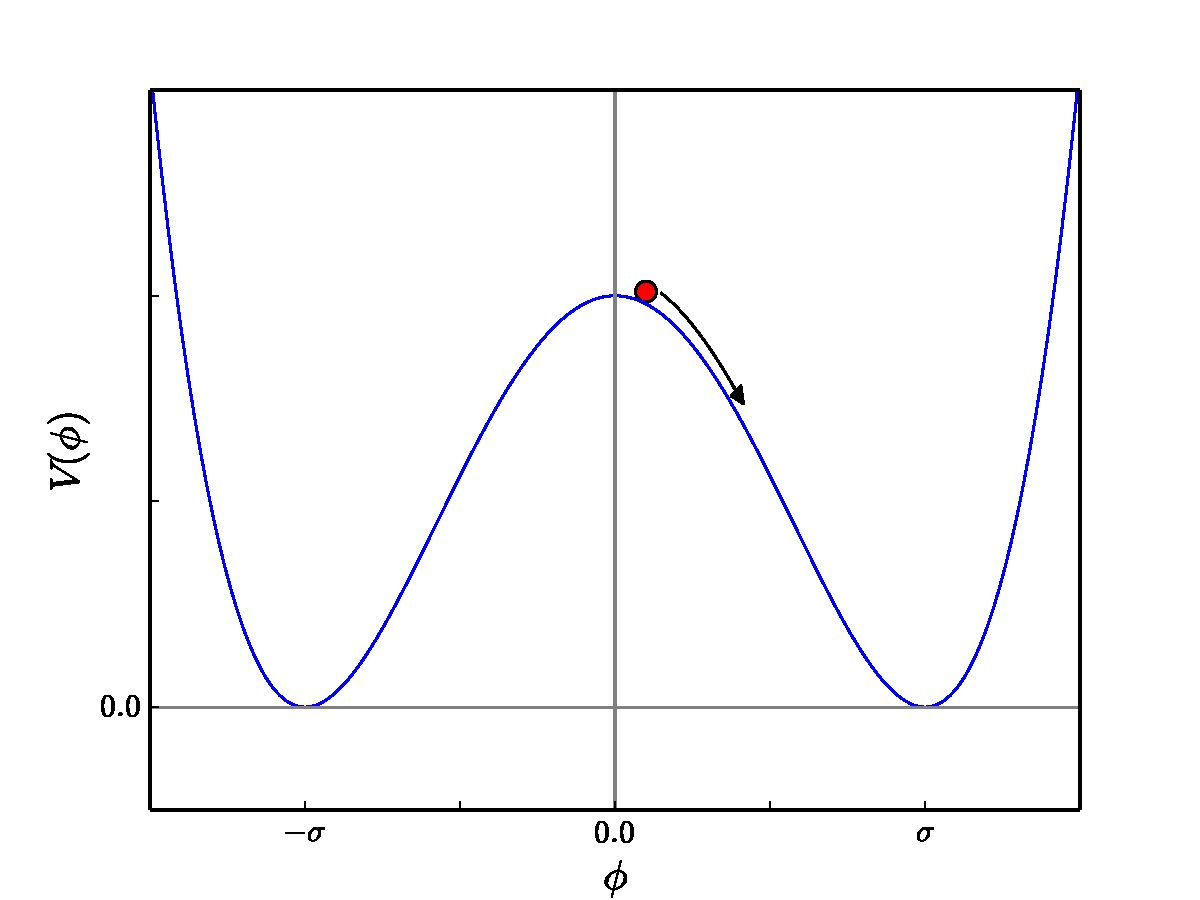
\includegraphics[width=0.50\textwidth]{figures/hilltop_cartoon.pdf}
	\caption{A schematic illustration of a hilltop potential, using the example of a Mexican Hat potential: $V(\phi)=\lambda(\phi^2-\sigma^2)^2$. The red ball symbolizes the inflationary field at a given time. The field rolls down the hill of the potential and settles in the vacuum state where the potential is zero, causing inflation to end. Note that in this scenario, the most inflation occurs at small values of $\phi$ and hence any hilltop model can be reasonably approximated by the first few lowest order terms.}
	\label{fig:MexHatCartoon}
\end{figure}

\begin{figure}[h]
	\centering
	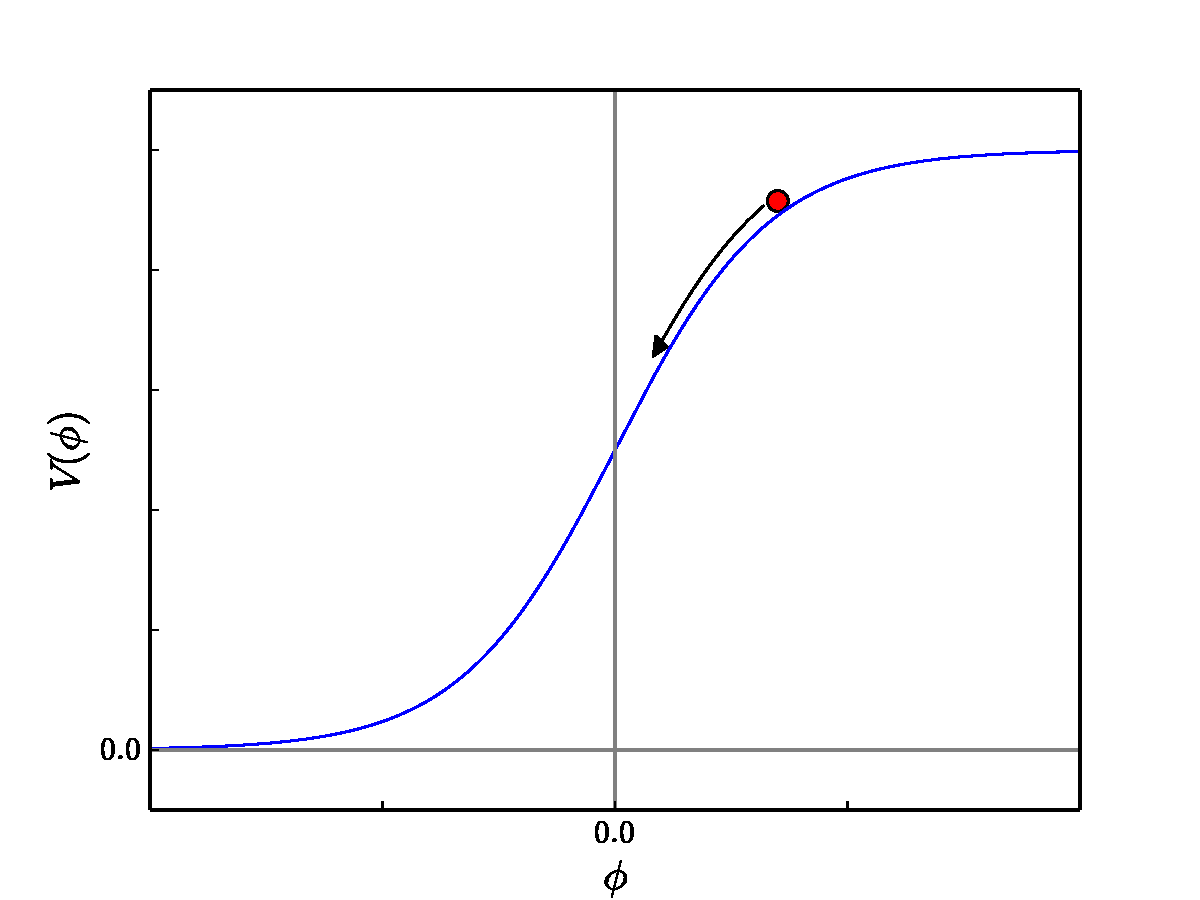
\includegraphics[width=0.50\textwidth]{figures/plateau_cartoon.pdf}
	\caption{A schematic illustration of a plateau potential. The red ball symbolizes the inflationary field at a given time. The field rolls down the hill of the potential and settles in the vacuum state where the potential is zero, causing inflation to end. Note that in this scenario, the most inflation occurs at large values of $\phi$. Therefore, unlike in the hilltop case, the highest order terms will dominate.}
	\label{fig:PlateauCartoon}
\end{figure}

The main purpose of an inflationary theory is to provide a mechanism to explain the homogeneity, isotropy, and flatness of the universe. As such, it is useful to look at the production of density perturbations during the inflationary period. During inflation, the magnitude of the density perturbations are inversely proportional to $\dot \phi$. Consequently, in regions where the potential is approximately constant, the perturbations would be unacceptably large. However, steeply-sloped potentials would cause the field to roll off the hill and end inflation before enough expansion took place. Therefore, there is a balancing game to be played in picking potentials. 

As we will see in the sections to come, this game of picking potentials to predict observations stumbles across many obstacles. Since the introduction of inflationary theory 34 years ago, many inflationary potentials have been proposed. However, once they satisfy observations, we have no natural criteria for choosing which among them is the ``true'' potential describing the inflationary field. 

In this paper we explore in the manner of \citet{Boyle+2006} a method of quantifying the amount of fine-tuning in an inflationary potential by counting the number of zeros in the equation of state and its derivatives. We find that \hl{...} We also explore a new method of quantifying the amount of fine-tuning in large field models that takes into account the sensitivity of the model to perturbations in higher-order terms. We find that \hl{...}

\subsection{History of Inflationary Theory}
\label{ssec:History}
Inflationary theory was first proposed by Alan Guth as a possible solution to the horizon and flatness problems \citep{Guth1981}. At the time, the standard cosmological model of the early universe was an adiabatically expanding, radiation-dominated universe. This model had two fundamental problems: the horizon problem and the flatness problem, discussed in more detail in Sections \ref{ssec:horizon} and \ref{ssec:Flatness}. Guth's inflationary model, which proposed a period of exponential expansion in a false vacuum due to supercooling during cosmological phase transitions, solved both the horizon and flatness problems.  However, later work by Guth and Weinberg \citep{Guth+Weinberg1983} showed that the transition could not be smoothly completed in such a way that would result in a space homogeneously filled with the new phase. Further, a random region within the inhomogeneous space would be unlikely to resemble our own universe. 

Andre Linde addressed these problems with a new inflationary theory in which inflation doesn't occur at the false vacuum but rather as the inflationary field rolled down the hill of the potential towards the true vacuum. \mep{Find Citation to presentation in 1981} A similar theory was simultaneously developed by \citet{Albrecht+Steinhardt1982}. This new inflation resolved the problem of the inhomogeneities because, as mentioned in Section \ref{ssec:GeneralDescription}, density fluctuations are inversely proportional to $\dot \phi$. Guth's previous model resulted in deSitter expansion, which corresponds to $\phi=const$, and hence results in unphysically large density fluctuations. Since in this new model inflation occurs as the field rolls down the hill, $\dot \phi \neq 0$ and perturbations can be made small enough to be physical. 

Although the new inflationary model solved some of the problems with Guth's original proposal, new inflation still came with issues of its own. For instance, the inflation field in the new theory often could not begin in thermal equilibrium with other fields, invalidating the use of cosmological phase transitions, which formed the basis of new inflation theory \citep{Linde2000}. Also, in the new inflationary scenario, inflation can only begin after at a time at least six orders of magnitude later than the Planck time, which is the order of a typical lifetime for a hot, closed universe \citep{LindeBook2005}. These problems, together with others, suggested that new inflation needed to be replaced with an even newer theory. 



\subsection{Horizon Problem}
\label{ssec:horizon}
Simply put, the horizon problem is the realization that the universe is homogenous and isotropic on scales far larger than the particle horizon (the farthest distance from which a point could ever receive information, given the age and expansion rate of the universe). The particle horizon is defined as 
\begin{equation}
d_p(t) = a(t) \int_0^t \frac{\d t}{a(t)},
\label{eqn:particle_horizon}
\end{equation}
where $a(t)$ is the scale factor of the universe, normalized to 1 at the present time. Consider a radiation-dominated universe, which is governed by the Friedmann equation:
\begin{equation}
H^2 = \left ( \frac{\dot a(t)}{a(t)} \right ) ^2 = \frac{8 \pi G}{3} \frac{\rho^0_r}{a^4}.
\end{equation}
Integrating this equation finds $a(t) \propto t^{1/2}$. Putting this into equation (\ref{eqn:particle_horizon}) finds that $d_p(t) = 2t \propto a^2$. Now, the size of any homogenous region is proportional to $a$. Therefore, at very small times (e.g. the Planck time), the size of the particle horizon will necessarily be smaller than the size of any homogenous region. This is a problem because, in order for a homogenous region to make sense, there must be a time at which the size of the homogenous region was smaller than the particle horizon. 

Observations of the CMB show the universe to homogenous to [Insert ridiculously small scale here], giving the homogenous region a size $l \sim c t_*$, where $t_*$ is the age of the universe at decoupling. The size of the homogenous region it must have originated from must have a size greater than $l_i \sim c t_* \tfrac{a_i}{a_*}$. However, the size of the particle horizon at that time was $l_h \sim c*t_*$. Therefore, comparing the two sizes, we find
\begin{equation}
\frac{l_i}{l_h} \sim \frac{a_i}{a_*} \sim \frac{T_*}{T_i}.
\end{equation}
 Taking $T_i$ to be the Planck temperature ($\sim 10^{32}$K) and $T_* \sim $

\subsection{Flatness Problem}
\label{ssec:Flatness}

\section{Derivation of an Inflationary Theory}
\subsection{Inflationary Friedmann equation}
\label{ssec:InflationaryFriedmann}
To see how one could implement an inflationary theory, let us first examine a non-inflationary Friedmann equation:
\begin{equation}
H^2 = \left ( \frac{\dot a(t)}{a(t)} \right ) ^2 = \frac{8 \pi G}{3} \left [ \frac{\rho^0_m}{a^3} + \frac{\rho^0_r}{a^4} + \Lambda + \frac{\sigma^2}{a^6} + \frac{K}{a^2} \right ]
\end{equation}
where $\rho^0_m$ is the energy density of matter in the universe at time $t=0$ (set to be the present time), $\rho^0_r$ is the current energy of radiation, $\Lambda$ is the cosmological constant, $\sigma$ is the cosmic anisotropy term, and $K$ is the curvature of the universe. As we can see by examining the powers of $a$ in each term, the early universe is dominated by the anisotropy term, $\propto a^{-6}$, while the late universe is dominated by the curvature term (and cosmological constant). Therefore, the simplest way to add inflation to the model of the universe is to add an inflationary term to the Friedmann equation: 
\begin{equation}
H^2 = \left ( \frac{\dot a(t)}{a(t)} \right ) ^2 = \frac{8 \pi G}{3} \left [ \frac{\rho^0_m}{a^3} + \frac{\rho^0_r}{a^4} + \Lambda + \frac{\sigma^2}{a^6} + \frac{K}{a^2} + \frac{\rho^0_\phi}{a^{2\epsilon}} \right ]
\end{equation}
where $\rho^0_\phi$ is the energy density of the inflationary field and $\epsilon$ is a positive exponent. In order to ensure that the universe expands during the inflationary period, we must constrain the value of $\epsilon$. 
%that must satisfy $\epsilon<1$ for inflation to dominate in the early universe. (Note: $\epsilon>3$ would cause contraction in the early universe.) 
%\mep{I have in my notes that $\epsilon<1$ for inflation and $\epsilon>3$ for contraction, but that doesn't make sense, so I think that's wrong.} 
%Now using this form for the inflationary term, 
To do so, we must examine how an inflation-dominated universe would evolve. In a $\phi$-dominated universe, the Friedmann equation becomes:
\begin{equation}
H^2 = \left ( \frac{\dot a}{a} \right ) ^2 = \frac{H_0 \Omega_\phi}{a^{2\epsilon}},
\label{eqn:Friedmann_phi}
\end{equation}
where $H_0$ is the Hubble constant and $\Omega_\phi = \tfrac{8\pi G \rho_\phi}{3 H_0}$. Now, solving this equation for $a(t)$ gives
\begin{equation}
a(t) \propto (\epsilon \sqrt{H_0 \Omega_\phi} t)^{1/\epsilon},
\label{eqn:inflation_a(t)}
\end{equation}
and hence 
\begin{equation}
\ddot a(t) \propto \left ( \frac{1-\epsilon}{\epsilon} \right ) (H_0 \Omega_\phi)^{1/2\epsilon} t^{\tfrac{1-2\epsilon}{\epsilon}}. 
\end{equation}
From this, we can see that the condition for an expanding universe is $\epsilon<1$. 
%\mep{Shoot. So my notes must have been right. But how can a small power in the denominator dominate at small values of a? That doesn't make sense!?!? Also, I know for a fact that the radiation term dominates before matter. So to be consistent with that, higher (negative) powers dominate earlier.} 
However, note that at arbitrarily early times (small values of $a$), the anisotropy term will dominate. Thus, in order for inflation to dominate during early times, the value of $\rho^0_\phi$ compared to $\sigma^2$ and the other coefficients must be specified such that at the Planck scale the inflationary term will dominate. %Therefore, we want to find an inflationary theory that produces an inflationary term in the Friedmann equation $\propto a^{-2\epsilon}$ so that the universe will be dominated by expansion at early times. 
Also, it is important to note that, in order for inflation to end, $\epsilon$ must grow to become greater than one, so we know that $\epsilon$ should be time-dependent. 

\subsection{Inflationary Field \& Equation of State}

In order to derive a field theory that will produce such an inflationary term consistent with the requirements detailed in Section \ref{ssec:InflationaryFriedmann}, we turn to the equation of state, $w=\rho/p$, where $\rho$ is the energy density and $p$ is the pressure of the field. The equation of state is related to $\epsilon$ by the equation 
\begin{equation}
\epsilon = \tfrac{3}{2}(w+1). 
\label{eqn:eps_w}
\end{equation}
Thus, an inflationary field must have an equation of state $w<-1/3$. Table \ref{tab:field_scenarios} summarizes the values $w$ and $\epsilon$ and the evolution of $a(t)$ for different types of fields. 

\begin{table}[htbp]
   \centering
   \begin{tabular}{@{} lcccc @{}} % Column formatting, @{} suppresses leading/trailing space
      \toprule
      Field Type & $w=\rho/p$ &  $\epsilon=\tfrac{3}{2}(w+1)$ & $a(t)$ & $\ddot a(t)$ \\
      \midrule
      matter & 0 & $3/2$ & $\propto t^{2/3}$ & $>0$ \\
       radiation & $1/3$ & $2$ & $\propto t^{1/2}$ & $<0$ \\
       $\Lambda$ & $-1$ & $0$ & $\propto e^t$ & $>0$ \\
       inflation & $<-1/3$ & $<1$ & $\propto t^{1/\epsilon}$ & $>0$ \\
       contraction & $>1$ & $>3$ & $\propto t^{1/\epsilon}$ & $<0$ \\
      \bottomrule
   \end{tabular}
   \caption{The values of $w$ and $\epsilon$ and the evolution of $a(t)$ for different types of fields.}
   \label{tab:field_scenarios}
\end{table}


From Table \ref{tab:field_scenarios}, we see that an inflationary field must have an equation of state $w<-1/3$. From this, we want to put constrains on the Lagrangian density $\L$ for the inflationary field. Let $\phi$ be an inflationary field. Its Lagrangian density takes the form:
\begin{equation}
\L = -\half ( \partial_\mu \phi)^2 - V(\phi)
\end{equation}
Using the assumptions that $\phi$ is homogenous (so that $\partial_j \phi = 0$) and isotropic (so that we can use the Minkowski metric $\eta_{\mu\nu}$), we find that the stress-energy tensor of the field is
\begin{equation}
T_{\mu\nu} = -\eta_{\mu 0} \dot \phi^2 + \eta_{\mu\nu}(\half\dot \phi^2+V(\phi)).
\end{equation}
From this, we find that the equation of state is
\begin{equation}
w = \frac{\half \dot \phi^2 - V(\phi)}{\half \dot \phi^2 + V(\phi)}.
\label{eqn:w}
\end{equation}
Putting in the constraint on $w$ for inflation, we find that an inflationary field must satisfy 
\begin{equation}
\dot \phi^2 < V(\phi).
\end{equation}
\mep{Is this important? It seems it should be, but we never talked about it before...}

Once we have $\L$, we know that the equation of motion for the field is the Klein-Gordon equation:
\begin{equation}
\ddot \phi + 3H \dot \phi + V'(\phi) = 0,
\label{eqn:KG}
\end{equation}
where $H$ is the Hubble parameter, $V(\phi)$ is the inflationary potential, and a dot indicates a time derivative. In our convention, the reduced Planck mass is set to one, i.e. $M_{pl} = (8\pi G)^{-1/2} \equiv 1$. Combining this with the Friedmann equation, 
\begin{equation}
H = \sqrt{\tfrac{1}{3} \left ( \half \dot \phi^2 + V(\phi) \right )},
\label{eqn:Friedmann}
\end{equation}
completely determines the evolution of a universe dominated by an inflationary potential $V(\phi)$. It will be useful later on to re-write the Friedmann equation in terms of $\epsilon$. Putting together equations (\ref{eqn:Friedmann_phi}) and (\ref{eqn:inflation_a(t)}), we find that
\begin{equation}
\epsilon = -\frac{\dot H}{H}
\label{eqn:Friedmann_epsilon}
\end{equation}
Note that, for general inflationary potentials, $\epsilon$ will not be constant in time. This is fortuitous since, in order for inflation to end, $\epsilon$ will have to go from a value greater than 1 to a value less than 1. We can also use this equation to further constrain the inflationary potential with a ``graceful exit'' condition. \mep{I think this is true. I need to look up more info \& elaborate.}

\subsection{Calculating Observable Parameters}
Of course, the whole point of creating an inflationary theory is to be able to reproduce observational data. When observations from experiments such as WMAP and Planck observe the early universe, they measure the power spectrum of density fluctuations in the primordial plasma. \mep{More elaboration on where these come from}

Instead of working in units of time, where the time at the end of inflation is difficult to pinpoint, we choose instead to work in terms of the number of e-folds until the end of inflation, defined as 
\begin{equation}
N = -\int_t^{t_{end}} H \d t \text{\ \ \ or\ equivalently\ \ \ } \d N = -H \d t. 
\label{eqn:defN}
\end{equation}
Note that $N$ runs backwards in time, so as time increases the number of e-folds decreases. In these units, the end of inflation is defined to occur at $N=0$, so at this time $\epsilon=1$. Current observations look at a narrow window centered on $N=60\equiv N_*$.  

Figure \ref{fig:density_fluctuations} shows a schematic of the density fluctuations as a function of the wavenumber of the fluctuations ($\log k\sim\tfrac{1}{N}$). If the fluctuations were purely scale invariant, then the curve would be a horizontal line, the amplitude of the fluctuations independent of their wave number. Since current observations see only a very limited range near $N_*$, so they focus on measuring (and we focus on predicting) the deviation from scale invariance at that point. This deviation is called the spectral tilt, denoted $n_s(k^*)$, where $k^*$ is the value of $k$ at $N_*$. Following the work of \citet{Wang+1997}, we use an approximation of the spectral index to first order in $\epsilon$:
\begin{equation}
n_s \approx 1 - 2\epsilon - \frac{\d \ln(\epsilon)}{\d N} + \mathcal{O}(\epsilon^2),
\label{eqn:ns_def}
\end{equation}
where the equation of state is treated as a function of the number of e-foldings instead of a function of time. 

In addition to the spectral tilt at $N_*$, observations can also constrain the tensor-to-scalar power ratio, typically denoted $r$. The tensor-to-scalar ratio is typically computed in the slow-roll approximation (See Section \ref{ssec:SlowRoll} for more details), and we follow the conventions of \citet{Planck2013} to get 
\begin{equation}
r \approx 16 \epsilon.
\end{equation}


\subsection{Fine-tuning in an Inflationary Theory}
Now that we have the basic mechanics of an inflationary theory, we see that defining an instance of an inflationary theory reduces to defining the inflationary potential $V(\phi)$. In order for inflation to be a predictive theory, we need to find a way to choose which potentials are reasonable and then find whether any of those potentials would generate a universe that conforms with observations. 


\section{Eqns for Code}
Let $\phi$ be an inflationary field governed by equations (\ref{eqn:Friedmann}) and (\ref{eqn:KG}). For the purposes of our code, we find it easier to work with $\phi$ not as a function of time but rather as a function of the number of e-folds until the end of inflation, defined in equation (\ref{eqn:defN}). If we let $\phi'$ denote the derivative of $\phi$ with respect to $N$, so that $\dot \phi = -H \phi'$ the Friedmann equation becomes
\begin{equation}
H^2 = \frac{V(\phi)}{3 - \half(\phi')^2},
\end{equation}
and the Klein-Gordon equation becomes 
\begin{equation}
2H^2\phi'' + H^2(\phi')^3 - 6H^2\phi' + 2V'(\phi) = 0.
\label{eqn:KG_N}
\end{equation}

\subsection{Slow Roll Approximation}
\label{ssec:SlowRoll}
In the slow roll approximation, we assume that $\dot \phi$ and $\ddot \phi$ are small. In order for this to be true, the inflationary potential must not be varying rapidly, leading us to the slow roll approximations:
\begin{equation}
\left | \frac{V'(\phi)}{V(\phi)} \right | <<1 \text{\ \ \ and\ \ \ } \left | \frac{V''(\phi)}{V(\phi)} \right | <<1 .
\label{eqn:SlowRollApprox}
\end{equation}
With these approximations, the Friedmann equation becomes
\begin{equation}
3 H^2 \approx_{sr} V(\phi),
\label{eqn:Friedmann_sr}
\end{equation}
and the Klein-Gordon equation becomes
\begin{equation}
3 H \dot \phi \approx_{sr} -V'(\phi)
\label{eqn:KG_sr}
\end{equation}
We use these approximations to find the initial conditions for integrating equation (\ref{eqn:KG_N}): $\phi(N=0)$ and $\dot \phi(N=0)$. To do this, we use the fact that, at the end of inflation (i.e. at $N=0$), $\epsilon = 1$. Recall from Section \ref{ssec:InflationaryFriedmann} that the condition for accelerated expansion is $\epsilon<1$. Therefore, as the universe transitions out of the inflationary epoch and into a period of decelerating expansion (where $\epsilon>1$), there must be a point where $\epsilon=1$, marking the end of inflation. Putting together equations (\ref{eqn:eps_w}) and (\ref{eqn:w}), we find that 
\begin{equation}
\epsilon = \frac{3}{2} \left ( \frac{\dot \phi^2}{\half \dot \phi^2 + V(\phi)} \right ) \approx_{sr} \half \left (\frac{V'(\phi)}{V(\phi)} \right ) ^2 
\end{equation}
where we have used the slow roll approximations $\half \dot \phi^2 << V(\phi)$ and equation (\ref{eqn:KG_sr}). Setting $\epsilon=1$ gives us an equation we can solve for $\phi(N=0)$. Once we have $\phi(N=0)$, we can easily us equation (\ref{eqn:KG_sr}) to find $\dot \phi(N=0)$. 

\bibliographystyle{apj}
\bibliography{thesis}{}

\end{document}